%!TEX root = ../report.tex
\section{Fitting}
This section discusses fitting the \sindist{} over 2 kinds of statistical objects -- MSMs (moment summary measures), and PDFs, in an attempt to demonstrate its flexibility.

It is to be noted that since the \sindist{} is a location-scale family, investigating its fitting flexibility over standardized/normalized statistical objects is good enough, since it can always adapt to location-scale transformed analogues of the aforesaid objects.

\subsection{MLE, Score equations}
The score equations for maximum likelihood estimation of the parameters of the \sindist{} $\Sinu(a,d,s,k)$ are not analytically solvable, as we detail below. Consider $X_i \iidsim \Sinu(a,d,s,k) \quad \forall i=1(1)n$. The joint log-likelihood is:
\begin{equation*}
    l(a,d,s,k; \utilde x)
    = -n\ln(d)-n\ln(A(s,k)) + k\sum_{i=1}^n \ln \sin \pi\left( x_i-a \over d \right)^s
\end{equation*}
Denote $z_i = \frac{x_i -a}{d}$. Some preliminary calculation:
\begin{align*}
    \nabla_s A &= \pi k \int_0^1 \sin^{k-1}(\pi z^s) \cos(\pi z^s) (\ln z) z^s \ \d z\\
    \nabla_k A &= \int_0^1 \sin^k(\pi z^s) \ln \sin(\pi z^s) \ \d z
\end{align*}
Gives us the score equations:
\begin{align*}
    &\nabla_a \ell = 0 \iff \sum_{i=1}^n z_i^{s-1} \cot(\pi z_i^s) = 0;  && \nabla_d \ell = 0 \iff \pi sk \sum_{i=1}^n z_i^s \cot(\pi z_i^s) = -n \\
    &\nabla_s \ell = 0 \iff  \pi k \sum_{i=1}^n {z^s \cos \pi z^s \ln z  \over \sin \pi z^s} = n {\nabla_s A \over A};  &&  \nabla_k \ell = 0 \iff \sum_{i=1}^n \ln \sin \pi z_i^s = n{\nabla_k A \over A}
\end{align*}
which may not be solved analytically. It may be wise to abandon this approach in favour of maximizing the joint likelihood through numerical computation means.

\subsection{MSM on MSM}
Given a set of 4 moment summary measures (MSMs), we focus on the problem of fitting an appropriate \sindist{} to them, so that its MSMs match the specifications as closely as possible. Because $\Sinu(a,d,s,k)$ is a location-scale family in $(a,d)$, implying that its first two MSMs (mean \& variance) can be freely adjusted by modifying $(a,d)$ alone, it should be sufficient to investigate the skewness-kurtosis adaptability of the distribution through its parameters $s$ and $k$. Hence, choosing the Standard $\Sinu(s,k)$ family, we analyze its skewness-kurtosis cover in \autoref{fig:skewkurtcover} over a finite grid of parameter choices: $s,k = 0.05\,(0.05)\, 6$. The plot is colorized to indicate the choice of parameters as denoted in the legend aside.

\begin{figure}[h]
    \centering
    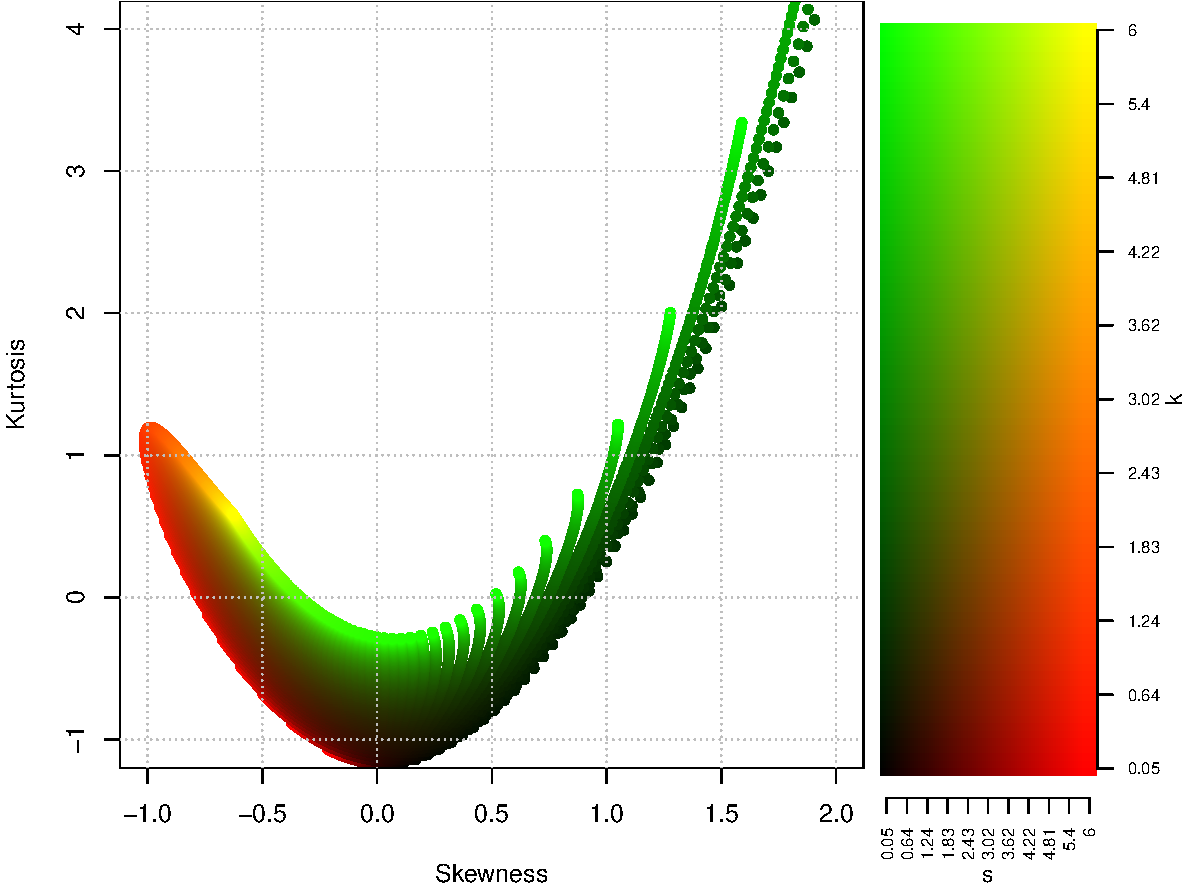
\includegraphics[width=0.8\linewidth]{fig/2-skewkurtcover}
    \caption{Skewness-Kurtosis cover of the \sindist.}
    \label{fig:skewkurtcover}
\end{figure}

At a later stage, we will assess the prospect of optimizing some distance metric over MSMs and open the path to numerical optimization.


\subsection{PDF on PDF}
We tried fitting the PDF of $\Sinu(a,d,s,k)$ over different target PDFs (standard location-scale members only) using numerical optimization (\texttt{L-BFGS-B} method of the \texttt{optim} function found in the \texttt{R} programming language) and the loss function as Hellinger distance. For finiteness of computation, we operate under the following parametric constraints whilst choosing the best candidate $\Sinu(a,d,s,k)$: $a \in [-10^3, 10^3]$, $d \in [10^{-2}, \, 2\times10^3]$, $s \in [10^{-2}, 10^2]$ and $k \in [10^{-2}, 10^2]$.
The results (minimized Hellinger distance with the choice of parameters) are provided in \autoref{tab:fitpdf}.
\begin{table}[h!]
    \centering
    \begin{tabularx}{\textwidth}{X|c}
        \toprule
        Target Density & Hellinger distance (Choice of Parameters $a,d,s,k$)\\
        \midrule
        $\N(0,1)$ & 0.00004277289 (-20.542932, 34.985498, 1.304535, 100)\\
        $\mathrm{Lognormal}(0,1)$ & 0.000936801 (0.02827762, 1000, 0.08566970, 35.78972) \\
        $\mathrm{Skew}\N_{\alpha=1} (0,1)$ & 2.189446e-05 (-7.2216216, 24.8516728, 0.5936823, 100) \\
        \hline
        $\mathrm{Logistic}(0,1)$ & 0.003149183 (-80.275639, 102.222513, 2.882431, 100) \\
        $\mathrm{Exp}(1)$ & 0.008101119 (0.0005708485, 6.5585684475, 0.0621246472, 1.6766166256) \\
        $\mathrm{DE}(0,1)$ & 0.01599712 (-8.895071, 16.872288, 1.085768, 15.608238) \\
        \hline
        $\Gamma(0.1,1)$ & Poor fit \\
        $\Gamma(100,1)$ & Poor fit \\
        $\Beta(1,1)$ & 0.0030202, (-0.0007780335, 1.0012066335, 0.1004892336, 0.12190192670) \\
        \hline
        $\mathrm{Cauchy}(0,1)$ & 0.06878475 (-126.211809, 149.303341, 4.141315, 100) \\
        \hline
        $\chi^2(1)$ & Poor fit \\
        $\chi^2(10)$ & 5.791378e-06 (-0.3201950, 97.1337699, 0.2815837, 22.0271292) \\
        $\mathrm{t}_1(0,1)$ & 0.06878477 (-126.114092, 149.207078, 4.138119, 100) \\
        $\mathrm{t}_{10}(0,1)$ & Fit failed \\
        $\mathrm{F}(1,1)$ & Poor fit \\
        \bottomrule
    \end{tabularx}
    \caption{Some common target densities and the best candidate \sindist{}}
    \label{tab:fitpdf}
\end{table}

The technical and theoretical underpinnings behind poor or failed fits will be the matter of future investigation.

\subsection{Mode matching}
WLoG, assume density is supported on $0,1$. Steps:
\begin{enumerate}
	\item Equate $2^{-1/s} = \text{given mode}$. Call the solution $s^*$.
	\item Equate $A(s^*, k) = \text{modal density}$. Call the solution $k^*$.
	\item Optimal density is $\Sinu(s^*, k^*)$. If this optimal density is a poor fit to the target, then either the target is not a Sinusoidal shape, or Sinusoidal distribution approximates is poorly within those bounds.
\end{enumerate}

\subsection{CDF on CDF}

\subsection{CDF on ECDF}

\subsection{QF on QF}
Quantile function on Quantile Function

\subsection{QF on EQF}

\subsection{DQF on DQF}



